\documentclass[11pt,a4paper]{article}

% ---------- Packages ----------
\usepackage[a4paper,margin=0.78in]{geometry}
\usepackage{setspace}
\usepackage{microtype}
\usepackage{graphicx}
\usepackage{booktabs}
\usepackage{array}
\usepackage{longtable}
\usepackage{tabularx}
\usepackage{multirow}
\usepackage{amsmath,amssymb}
\usepackage{xcolor}
\usepackage{hyperref}
\usepackage{enumitem}
\usepackage{caption}
\usepackage{subcaption}
\usepackage{float}
\usepackage{listings}
\usepackage{tcolorbox}
\usepackage{tikz}
\usetikzlibrary{arrows.meta,positioning,shapes.geometric,fit,calc}

\hypersetup{colorlinks=true,linkcolor=blue!55!black,urlcolor=blue!65!black,citecolor=blue!55!black}
\setstretch{1.08}
\setlist[itemize]{leftmargin=1.1em,itemsep=2pt,topsep=3pt}
\setlist[enumerate]{leftmargin=1.4em,itemsep=2pt,topsep=3pt}
\setlength{\tabcolsep}{4pt}
\emergencystretch=3em
\newcolumntype{Y}{>{\raggedright\arraybackslash}X}

% ---------- Colors ----------
\definecolor{eduNavy}{HTML}{0B1120}
\definecolor{eduBlue}{HTML}{2563EB}
\definecolor{eduTeal}{HTML}{14B8A6}
\definecolor{eduOrange}{HTML}{F59E0B}
\definecolor{eduGreen}{HTML}{16A34A}
\definecolor{eduGray}{HTML}{F3F4F6}
\definecolor{codeBg}{HTML}{F8FAFC}
\definecolor{codeFrame}{HTML}{CBD5E1}

\newtcolorbox{findingbox}{colback=blue!3!white,colframe=eduBlue!60!black,arc=2mm,boxrule=0.6pt,left=6pt,right=6pt,top=6pt,bottom=6pt}
\newtcolorbox{contribbox}{colback=teal!3!white,colframe=eduTeal!70!black,arc=2mm,boxrule=0.6pt,left=6pt,right=6pt,top=6pt,bottom=6pt}
\newtcolorbox{cautionbox}{colback=orange!5!white,colframe=eduOrange!75!black,arc=2mm,boxrule=0.6pt,left=6pt,right=6pt,top=6pt,bottom=6pt}

\lstdefinestyle{promptstyle}{
  backgroundcolor=\color{codeBg},
  basicstyle=\ttfamily\scriptsize,
  frame=single,
  rulecolor=\color{codeFrame},
  breaklines=true,
  columns=fullflexible,
  keepspaces=true,
  showstringspaces=false,
  aboveskip=6pt,
  belowskip=6pt
}
\lstset{style=promptstyle}

% ---------- TikZ styles ----------
\tikzset{
  proc/.style={rectangle, rounded corners=2pt, draw=eduBlue!65!black, fill=blue!5, align=center, minimum width=3.3cm, minimum height=0.78cm, font=\scriptsize},
  agent/.style={rectangle, rounded corners=2pt, draw=eduOrange!75!black, fill=orange!8, align=center, minimum width=3.3cm, minimum height=0.78cm, font=\scriptsize},
  data/.style={rectangle, rounded corners=2pt, draw=eduGreen!65!black, fill=green!6, align=center, minimum width=3.3cm, minimum height=0.78cm, font=\scriptsize},
  store/.style={cylinder, shape border rotate=90, aspect=0.24, draw=eduTeal!75!black, fill=teal!5, align=center, minimum width=2.8cm, minimum height=0.9cm, font=\scriptsize},
  decision/.style={diamond, aspect=1.9, draw=eduNavy!75, fill=eduGray, align=center, inner sep=1.2pt, font=\scriptsize},
  arrow/.style={-Latex, thick, draw=eduNavy!75}
}

\title{\vspace{-1.5cm}\textbf{EduAgent: A Personalized Agentic AI Tutor with Fine-Tuned Difficulty Classification, Semantic Two-Pass RAG, Learner Memory, Voice Interaction, and Adaptive Teaching Modes}\\[0.45em]
\large Research Paper-Style Technical Report}
\author{Department of Artificial Intelligence \\ Third Year B.Tech GenAI Project}
\date{May 2026}

\begin{document}
\maketitle

\begin{abstract}
EduAgent is a personalized AI/ML tutoring system that moves beyond one-shot chatbot behavior by combining a fine-tuned DistilBERT difficulty classifier, semantic topic detection, two-pass personalized retrieval, persistent learner memory, LLM-based tutoring and evaluation agents, and a Gradio interface with voice input/output. The updated repository uses a 2,400-row Gemini-generated instructional dataset with topic, subtopic, difficulty, angle, reasoning, and confusion metadata. A DistilBERT classifier trained on this dataset reaches 97.92\% test accuracy and 97.91\% macro-F1 on a balanced 240-example test split. The current saved RAG checkpoint evaluates 18 questions and reports Hit Rate@3 = 83.3\%, MRR = 0.8333, Topic Precision = 83.3\%, Level Precision = 100\%, average semantic similarity = 0.7153, Faithfulness = 5.00/5, Answer Relevancy = 5.00/5, Context Utilization = 4.44/5, and Level Fit = 4.94/5. A separate weak-area retrieval evaluation reports 100\% keyword relevance over five simulated learner weakness profiles. This report documents the architecture, dataset construction, prompts, classifier results, RAG evaluation, memory update equations, testing evidence, limitations, and future research directions.
\end{abstract}


\tableofcontents
\newpage

% =========================================================
\section{Introduction}

LLM-based educational assistants often answer the current question but do not reliably remember the learner, detect the learner's difficulty level, retrieve level-appropriate examples, check understanding, or adapt the next explanation. EduAgent addresses this limitation by wrapping LLM generation inside an agentic tutoring loop:

\[
\text{Ask} \rightarrow \text{Classify} \rightarrow \text{Retrieve} \rightarrow \text{Teach} \rightarrow \text{Evaluate} \rightarrow \text{Remember} \rightarrow \text{Adapt}.
\]

The updated EduAgent repository implements this loop as a working application rather than a static notebook. It includes authentication, SQLite-backed learner profiles, a local DistilBERT classifier, semantic retrieval using \texttt{all-MiniLM-L6-v2}, LLM-based Tutor and Evaluator agents, an adaptive Memory Agent, voice input/output modules, dashboard visualizations, and evaluation scripts.

\subsection{Main Research Contributions}

\begin{contribbox}
\begin{enumerate}
    \item \textbf{Dataset upgrade:} Replaced a compact 900-row baseline dataset with a 2,400-row metadata-rich AI/ML tutoring dataset: 25 topics $\times$ 4 subtopics $\times$ 3 difficulty levels $\times$ 8 examples.
    \item \textbf{Fine-tuned difficulty classifier:} Trained \texttt{distilbert-base-uncased} for 3-class difficulty prediction, achieving 97.92\% test accuracy and 97.91\% macro-F1.
    \item \textbf{Two-pass personalized RAG:} Pass 1 retrieves examples similar to the learner query; Pass 2 retrieves weak-area examples from the learner profile.
    \item \textbf{Adaptive teaching modes:} Four modes - default, remedial, clarification, and advance - are selected from evaluator output, mastery scores, weak concepts, and prior explanation styles.
    \item \textbf{Closed feedback loop:} Follow-up evaluation updates weak areas, mastery, recommendations, and the prompt strategy used in later turns.
    \item \textbf{Operational application:} The project includes authentication, SQLite persistence, Gradio UI, learner dashboard charts, voice input, voice output, retry-aware LLM client, and unit tests.
\end{enumerate}
\end{contribbox}

% =========================================================
\section{System Architecture}

\subsection{End-to-End Pipeline}

Figure~\ref{fig:pipeline} summarizes the updated repository workflow. Blue boxes are deterministic/system components, green boxes are retrieval and memory components, orange boxes are LLM agents, and cylinders represent persistent or reusable data stores.


\begin{figure}[H]
\flushleft
\resizebox{0.96\textwidth}{!}{%
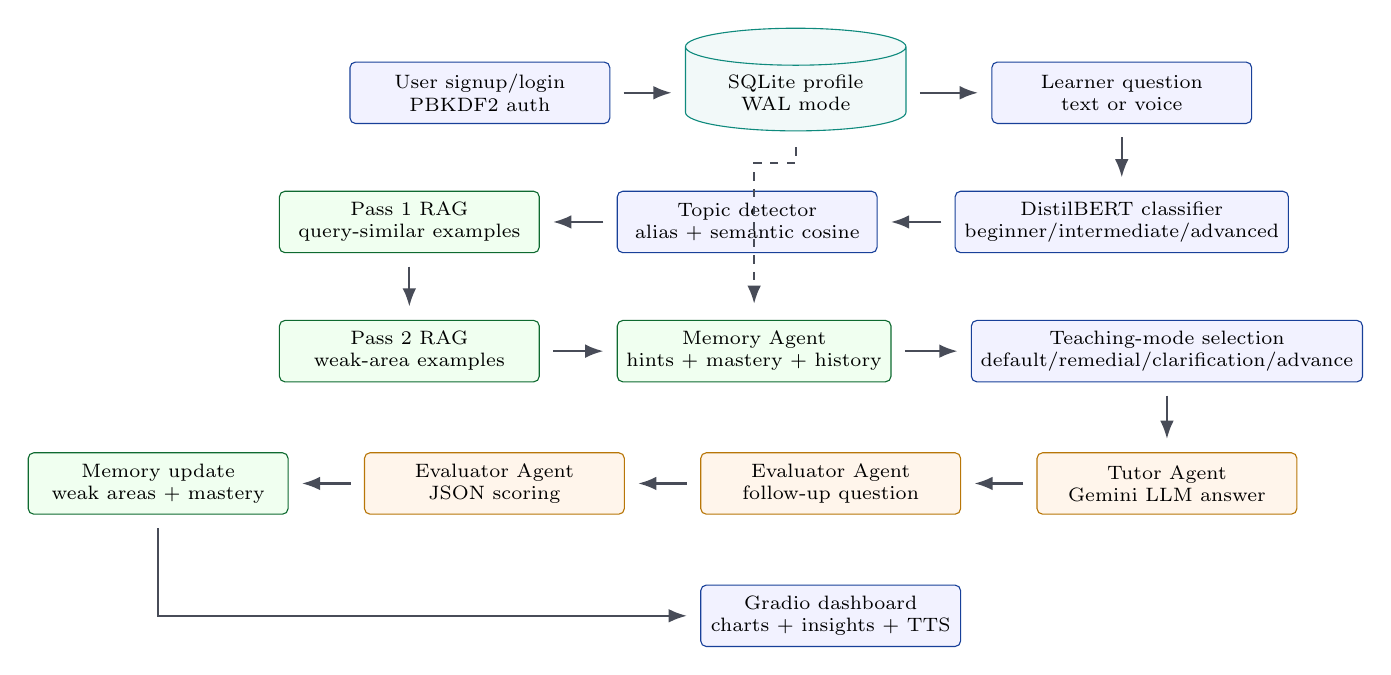
\begin{tikzpicture}[node distance=0.82cm and 0.78cm,every node/.style={outer sep=2pt}]

\node[proc] (login) {User signup/login\\PBKDF2 auth};
\node[store, right=0.82cm of login] (sqlite) {SQLite profile\\WAL mode};
\node[proc, right=0.95cm of sqlite] (question) {Learner question\\text or voice};

\node[proc, below=0.72cm of question] (clf) {DistilBERT classifier\\beginner/intermediate/advanced};
\node[proc, left=0.85cm of clf] (topic) {Topic detector\\alias + semantic cosine};
\node[data, left=0.85cm of topic] (rag1) {Pass 1 RAG\\query-similar examples};
\node[data, below=0.72cm of rag1] (rag2) {Pass 2 RAG\\weak-area examples};
\node[data, right=0.85cm of rag2] (memory) {Memory Agent\\hints + mastery + history};
\node[proc, right=0.88cm of memory] (mode) {Teaching-mode selection\\default/remedial/clarification/advance};

\node[agent, below=0.76cm of mode] (tutor) {Tutor Agent\\Gemini LLM answer};
\node[agent, left=0.83cm of tutor] (follow) {Evaluator Agent\\follow-up question};
\node[agent, left=0.83cm of follow] (score) {Evaluator Agent\\JSON scoring};
\node[data, left=0.83cm of score] (update) {Memory update\\weak areas + mastery};
\node[proc, below=0.76cm of follow] (dashboard) {Gradio dashboard\\charts + insights + TTS};

\draw[arrow,shorten >=3pt,shorten <=3pt] (login.east) -- (sqlite.west);
\draw[arrow,shorten >=3pt,shorten <=3pt] (sqlite.east) -- (question.west);
\draw[arrow,shorten >=3pt,shorten <=3pt] (question.south) -- (clf.north);
\draw[arrow,shorten >=3pt,shorten <=3pt] (clf.west) -- (topic.east);
\draw[arrow,shorten >=3pt,shorten <=3pt] (topic.west) -- (rag1.east);
\draw[arrow,shorten >=3pt,shorten <=3pt] (rag1.south) -- (rag2.north);
\draw[arrow,shorten >=3pt,shorten <=3pt] (rag2.east) -- (memory.west);
\draw[arrow,shorten >=3pt,shorten <=3pt] (memory.east) -- (mode.west);
\draw[arrow,shorten >=3pt,shorten <=3pt] (mode.south) -- (tutor.north);
\draw[arrow,shorten >=3pt,shorten <=3pt] (tutor.west) -- (follow.east);
\draw[arrow,shorten >=3pt,shorten <=3pt] (follow.west) -- (score.east);
\draw[arrow,shorten >=3pt,shorten <=3pt] (score.west) -- (update.east);
\draw[arrow,shorten >=3pt,shorten <=3pt] (update.south) |- (dashboard.west);

\draw[arrow,dashed,shorten >=4pt,shorten <=4pt] (sqlite.south) -- ++(0,-0.34) -| (memory.north);

\end{tikzpicture}}
\caption{EduAgent end-to-end architecture. The dashed arrow represents cross-turn profile reads.}
\label{fig:pipeline}
\end{figure}

\subsection{Repository Module Map}

\begin{longtable}{p{0.29\textwidth}p{0.63\textwidth}}
\toprule
\textbf{Module} & \textbf{Role in the system} \\
\midrule
\endhead
\texttt{config/settings.py} & Central configuration: Gemini key/model, dataset path, classifier path, DB file, RAG top-N values, evaluation model, retry settings. \\
\texttt{ml/classifier.py} & Loads local DistilBERT model from \texttt{models/distilbert\_eduagent\_v2}, falls back to Hugging Face repo, then heuristic classification. Adds calibration for beginner, comparison, and advanced-intent phrasing. \\
\texttt{ml/embedder.py} & Loads shared \texttt{all-MiniLM-L6-v2} embedder from local cache and exposes a singleton to avoid loading the sentence-transformer twice. \\
\texttt{ml/topic\_detector.py} & Detects canonical AI/ML topic using alias matching first, then semantic topic vectors or TF-IDF fallback. \\
\texttt{ml/retriever.py} & Implements level/topic filtering, semantic or TF-IDF retrieval, keyword overlap scoring, complexity penalty, and weak-area retrieval. \\
\texttt{agents/tutor\_agent.py} & Orchestrates classification, topic detection, Pass 1 RAG, Pass 2 RAG, memory hints, teaching-mode inference, prompt assembly, and answer generation. \\
\texttt{agents/evaluator\_agent.py} & Generates a conceptual follow-up question and evaluates learner replies into a validated schema: \texttt{good}, \texttt{partial}, or \texttt{poor}. \\
\texttt{agents/memory\_agent.py} & Maintains profile schema, updates topic counts, mastery, weak areas, used explanation tags, recommendations, and prompt hints. \\
\texttt{agents/llm\_client.py} & Wraps Gemini calls, OpenAI-style messages, retry logic, timeout, quota detection, and fallback behavior. \\
\texttt{auth/password\_utils.py} & PBKDF2-SHA256 password hashing with 16-byte salts and \texttt{hmac.compare\_digest}. \\
\texttt{db/sqlite\_store.py} & SQLite initialization with WAL mode, synchronous=NORMAL, users table, profiles table, and schema migration checks. \\
\texttt{db/profile\_repository.py} & User CRUD and profile JSON serialization/deserialization with safe JSON defaults. \\
\texttt{app/main.py} & Gradio callback orchestration: login, signup, question asking, follow-up evaluation, profile save, chart generation, retrieved-example display, voice callbacks. \\
\texttt{app/ui.py} & Full Gradio layout and CSS: auth hero, chat panel, dashboard cards, charts, retrieved examples, system insights, voice controls. \\
\texttt{voice/} & Whisper speech-to-text wrapper, local TTS wrapper using Piper if available or \texttt{pyttsx3} fallback, and UI utilities. \\
\texttt{eval/} and \texttt{rag\_evaluation.py} & Retrieval/generation evaluation, LLM-as-judge scoring, checkpointing, pass-2 weak-area evaluation. \\
\texttt{tests/} & Unit tests for authentication, profile normalization, and memory/mastery behavior. \\
\bottomrule
\caption{Updated repository module map.}
\end{longtable}

% =========================================================
\section{Dataset Construction and Quality}

\subsection{Dataset Used by the Updated Application}

The active dataset path in \texttt{config/settings.py} is:

\begin{lstlisting}
DATASET_FILE = str(BASE_DIR / "datasets" / "data_easy" / "eduagent_dataset_easy_v2.csv")
\end{lstlisting}

The submitted dataset has 2,400 rows and 19 columns. Its generation target is exactly balanced:

\[
25 \text{ topics} \times 4 \text{ subtopics} \times 3 \text{ levels} \times 8 \text{ examples} = 2400.
\]

\begin{table}[H]
\centering
\begin{tabular}{l r}
\toprule
\textbf{Property} & \textbf{Value in updated repo} \\
\midrule
Rows & 2,400 \\
Columns & 19 \\
Difficulty levels & beginner, intermediate, advanced \\
Rows per level & 800 each \\
Topics & 25 \\
Rows per topic & 96 each \\
Subtopics & 99 unique subtopic strings \\
Examples per topic-subtopic-level cell & 8 \\
Duplicate questions & 0 \\
Duplicate answers & 0 \\
Average question length & 22.60 words \\
Average answer length & 119.16 words \\
Generator provider/model & Gemini / \texttt{gemini-2.5-flash} \\
Prompt version stored in data & \texttt{eduagent\_easy\_batch\_v1} \\
\bottomrule
\end{tabular}
\caption{Dataset statistics computed from \texttt{datasets/data\_easy/eduagent\_dataset\_easy\_v2.csv}.}
\end{table}

\subsection{Metadata Schema}

The dataset is not only a question-answer set; it is a pedagogy-aware instruction dataset. Its columns include:

\begin{center}
\small
\begin{tabular}{p{0.30\textwidth}p{0.60\textwidth}}
\toprule
\textbf{Column group} & \textbf{Examples} \\
\midrule
Identity and taxonomy & \texttt{id}, \texttt{topic}, \texttt{subtopic}, \texttt{level}, \texttt{question\_angle} \\
Instruction content & \texttt{question}, \texttt{answer} \\
Length diagnostics & \texttt{question\_word\_count}, \texttt{answer\_word\_count} \\
Pedagogical annotations & \texttt{key\_concepts}, \texttt{expected\_reasoning}, \texttt{difficulty\_rationale}, \texttt{why\_this\_fits\_level}, \texttt{concepts\_covered}, \texttt{possible\_learner\_confusion} \\
Generation metadata & \texttt{generator\_provider}, \texttt{generator\_model}, \texttt{prompt\_version}, \texttt{timestamp} \\
\bottomrule
\end{tabular}
\end{center}

These extra fields are useful for retrieval, reportability, curriculum-aware filtering, and future instruction-tuning experiments.

\subsection{Comparison with the Original 900-Row Dataset}

The updated dataset is substantially richer than the original 900-row dataset. The detailed analysis document reports the following structural comparison.

\begin{table}[H]
\centering
\begin{tabular}{lrr}
\toprule
\textbf{Metric} & \textbf{Dataset 1: 900 rows} & \textbf{Dataset 2: 2400 rows} \\
\midrule
Rows & 900 & 2,400 \\
Columns & 5 & 19 \\
Question avg. words & 22.0 & 22.6 \\
Answer avg. words & 62.13 & 119.16 \\
Question duplicate \% & 0.0 & 0.0 \\
Answer duplicate \% & 0.0 & 0.0 \\
Question vocabulary size & 2,025 & 3,706 \\
Answer vocabulary size & 4,474 & 8,273 \\
Metadata richness & Low & Very high \\
\bottomrule
\end{tabular}
\caption{Dataset comparison from the detailed dataset analysis, verified against the repository dataset where possible.}
\end{table}

\subsection{Batch Dataset Generation Pipeline}

The updated generator is \texttt{datasets/generate\_dataset\_v2.py}. It uses Gemini structured batch output but keeps deterministic local filters in the hot loop. The script design is documented in its header as follows: generate multiple candidate Q/A rows per topic-subtopic-level cell, apply local filters, save continuously to JSONL and CSV, and avoid model self-validation inside the hot loop to reduce wasted calls.

\subsubsection{Generation Taxonomy}

\begin{table}[H]
\centering
\small
\begin{tabular}{p{0.18\textwidth}p{0.72\textwidth}}
\toprule
\textbf{Level} & \textbf{Question angles in the updated generator} \\
\midrule
Beginner & definition with simple example; real-world analogy; why it matters; common misconception; basic comparison; high-level working; first learning step; simple consequence \\
Intermediate & implementation detail; trade-off analysis; debugging scenario; evaluation decision; dataset impact; workflow choice; comparison between methods; practical failure mode \\
Advanced & edge case analysis; scalability concern; theoretical intuition; research limitation; robustness concern; system design integration; probabilistic interpretation; complexity analysis \\
\bottomrule
\end{tabular}
\caption{Level-specific question-angle bank used by the generator.}
\end{table}

\subsubsection{Local Quality Filters}

The script enforces level leakage rejection, length bounds, duplicate/near-duplicate checks, and generic-pattern rejection for intermediate/advanced rows.

\begin{table}[H]
\centering
\begin{tabular}{lrr}
\toprule
\textbf{Level} & \textbf{Question word range} & \textbf{Answer word range} \\
\midrule
Beginner & 7--45 & 50--130 \\
Intermediate & 9--60 & 75--170 \\
Advanced & 11--75 & 95--230 \\
\bottomrule
\end{tabular}
\caption{Deterministic local length filters from the updated dataset generator.}
\end{table}

Near-duplicates are rejected when \texttt{SequenceMatcher} ratio $\ge 0.90$ or Jaccard token similarity $\ge 0.82$ within the same topic-subtopic-level cell.

\subsection{Dataset Generation Prompt}

The full prompt generated by \texttt{build\_batch\_prompt()} is parameterized by \texttt{topic}, \texttt{subtopic}, \texttt{level}, \texttt{candidate\_count}, and existing questions. The core template is:

\begin{lstlisting}
You are generating high-quality rows for an AI/ML tutoring dataset called EduAgent.

Generate {candidate_count} diverse candidate rows.
Only generate rows for this exact cell:
Topic: {topic}
Subtopic: {subtopic}
Difficulty level: {level}

Existing questions to avoid:
{existing_block}

Use these angles across the rows where possible:
{angles}

Hard quality rules:
- Each question must be specific, useful, and end with a question mark.
- Question length must be {q_min} to {q_max} words.
- Answer length must be {a_min} to {a_max} words.
- Do not mention the difficulty label in the question or answer.
- Do not write "For a beginner", "For an intermediate", or "For an advanced".
- Do not use markdown, bullets, numbered lists, tables, or code blocks.
- Avoid generic questions like "What is {subtopic}?" unless the beginner row adds context and learning value.
- Each answer must be factually correct, self-contained, and pedagogically useful.
- Questions must be meaningfully different from each other and from the existing questions.

Level expectations:
Beginner: simple explanation, intuitive example, no equations, minimal jargon.
Intermediate: practical reasoning, comparison, debugging, implementation, or evaluation.
Advanced: edge cases, assumptions, scalability, theory, robustness, or system design reasoning.

Return valid JSON only in this exact shape:
{
  "rows": [
    {
      "question": "...",
      "answer": "...",
      "question_angle": "...",
      "key_concepts": ["...", "..."],
      "expected_reasoning": "...",
      "possible_learner_confusion": "...",
      "difficulty_rationale": "...",
      "why_this_fits_level": "..."
    }
  ]
}
\end{lstlisting}

% =========================================================
\section{Difficulty Classification}

\subsection{Classifier Design}

The updated repository uses a local fine-tuned \texttt{distilbert-base-uncased} sequence classifier stored at:

\begin{lstlisting}
models/distilbert_eduagent_v2
\end{lstlisting}

The model predicts three labels: \texttt{beginner}, \texttt{intermediate}, and \texttt{advanced}. \texttt{ml/classifier.py} first attempts to load the local model. If local weights are unavailable, it attempts a Hugging Face Hub fallback via \texttt{CLASSIFIER\_HF\_REPO}. If both fail, the system falls back to deterministic heuristics. The classifier removes \texttt{token\_type\_ids} before inference because DistilBERT does not use segment embeddings.

\subsection{Training Configuration}

The saved \texttt{training\_config.json} in the repository records:

\begin{table}[H]
\centering
\begin{tabular}{ll}
\toprule
\textbf{Parameter} & \textbf{Value} \\
\midrule
Base model & \texttt{distilbert-base-uncased} \\
Epochs & 3 \\
Batch size & 8 \\
Max length & 128 \\
Learning rate & $2 \times 10^{-5}$ \\
Weight decay & 0.01 \\
Warmup ratio & 0.06 \\
Early stopping patience & 2 \\
Random seed & 42 \\
Train/validation/test split & 80/10/10 stratified by level \\
\bottomrule
\end{tabular}
\caption{Training configuration saved by the updated repository.}
\end{table}

The train/validation/test files saved in the model folder contain 1,920, 240, and 240 examples respectively.

\subsection{Classifier Results}

The repository classification report gives the following test-set performance:

\begin{table}[H]
\centering
\begin{tabular}{lrrrr}
\toprule
\textbf{Class} & \textbf{Precision} & \textbf{Recall} & \textbf{F1} & \textbf{Support} \\
\midrule
Beginner & 0.9875 & 0.9875 & 0.9875 & 80 \\
Intermediate & 0.9870 & 0.9500 & 0.9682 & 80 \\
Advanced & 0.9639 & 1.0000 & 0.9816 & 80 \\
\midrule
Accuracy & \multicolumn{3}{r}{0.9792} & 240 \\
Macro average & 0.9795 & 0.9792 & 0.9791 & 240 \\
Weighted average & 0.9795 & 0.9792 & 0.9791 & 240 \\
\bottomrule
\end{tabular}
\caption{Fine-tuned DistilBERT test performance.}
\label{tab:classifier-results}
\end{table}

The confusion matrix is:

\begin{center}
\begin{tabular}{lccc}
\toprule
& \textbf{Pred. beginner} & \textbf{Pred. intermediate} & \textbf{Pred. advanced} \\
\midrule
True beginner & 79 & 1 & 0 \\
True intermediate & 1 & 76 & 3 \\
True advanced & 0 & 0 & 80 \\
\bottomrule
\end{tabular}
\end{center}

Advanced examples are never misclassified as easier levels in the saved test split. Intermediate has the highest confusion, with three intermediate examples predicted as advanced.

\subsection{Calibration Layer}

The repository does not blindly trust the neural classifier in every case. It adds a small post-prediction calibration layer:

\begin{itemize}
    \item Short definition-style questions can be forced to beginner.
    \item Ordinary comparison questions can be treated as intermediate.
    \item Comparison questions with convergence, derivation, proof, formal, loss landscape, or complexity markers can be upgraded to advanced.
    \item Explicit advanced markers such as \texttt{derive}, \texttt{prove}, \texttt{theorem}, \texttt{convergence}, \texttt{architecture}, \texttt{attention mechanism}, \texttt{backpropagation}, and \texttt{gradient flow} can override raw predictions.
\end{itemize}

This makes the deployed classifier more robust to short and ambiguous real learner queries than a pure argmax classifier.

% =========================================================
\section{Semantic Topic Detection}

The topic detector uses a two-tier design:

\begin{enumerate}
    \item \textbf{Alias tier:} space-padded exact substring matching against a manually curated alias table. This handles terms such as \texttt{cnn}, \texttt{rag}, \texttt{llm}, \texttt{tfidf}, \texttt{transformer architecture}, and \texttt{bias mitigation}.
    \item \textbf{Semantic tier:} for each topic in the current level slice, the system builds a rich topic document of the form \texttt{topic name: all questions for that topic}. It encodes topic documents with the shared \texttt{all-MiniLM-L6-v2} embedder and selects the highest cosine-similarity topic when the score is convincing.
\end{enumerate}

If the sentence-transformer cannot load locally, the detector falls back to a TF-IDF topic index. If all similarity scores are too low, the default topic is selected from general topics such as machine learning basics, neural networks, or classification.

\begin{figure}[H]
\centering
\resizebox{0.86\textwidth}{!}{%
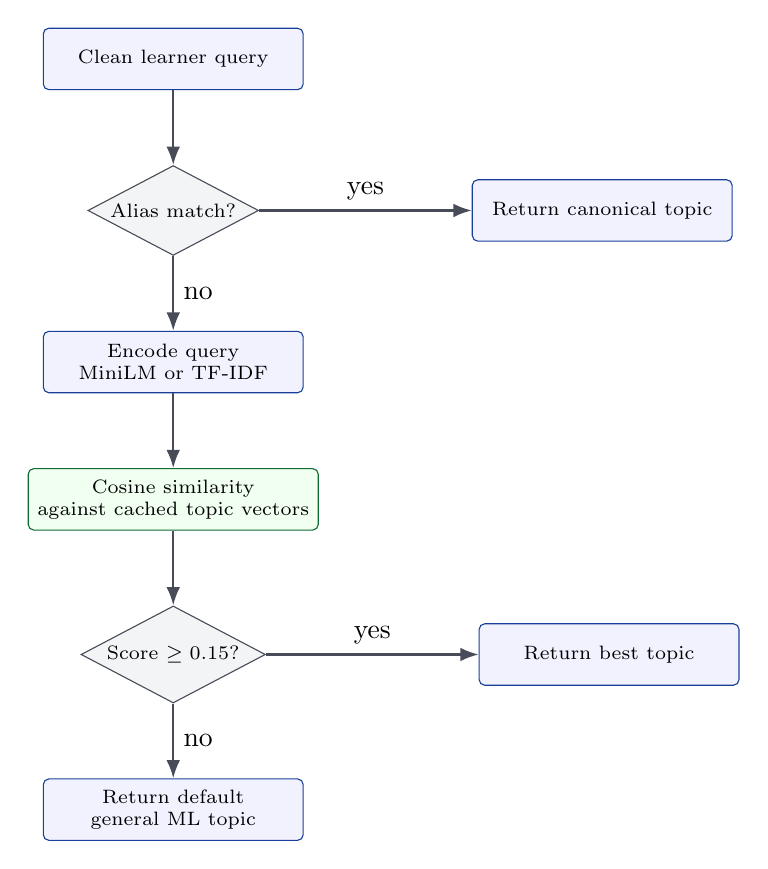
\begin{tikzpicture}[node distance=0.95cm]
\node[proc] (q) {Clean learner query};
\node[decision, below=of q] (alias) {Alias match?};
\node[proc, right=2.7cm of alias] (canonical) {Return canonical topic};
\node[proc, below=of alias] (encode) {Encode query\\MiniLM or TF-IDF};
\node[data, below=of encode] (compare) {Cosine similarity\\against cached topic vectors};
\node[decision, below=of compare] (threshold) {Score $\ge 0.15$?};
\node[proc, right=2.7cm of threshold] (best) {Return best topic};
\node[proc, below=of threshold] (default) {Return default\\general ML topic};
\draw[arrow] (q) -- (alias);
\draw[arrow] (alias) -- node[above]{yes} (canonical);
\draw[arrow] (alias) -- node[right]{no} (encode);
\draw[arrow] (encode) -- (compare);
\draw[arrow] (compare) -- (threshold);
\draw[arrow] (threshold) -- node[above]{yes} (best);
\draw[arrow] (threshold) -- node[right]{no} (default);
\end{tikzpicture}}
\caption{Updated two-tier topic detection: alias matching followed by semantic or TF-IDF fallback.}
\end{figure}

% =========================================================
\section{Two-Pass Personalized RAG}

\subsection{Pass 1: Query-Similar Educational Retrieval}

\texttt{ml/retriever.py} loads the active dataset once and caches an index for each \texttt{(level, topic)} slice. For semantic retrieval, it encodes questions using \texttt{all-MiniLM-L6-v2}. If sentence-transformers are unavailable, the app falls back to TF-IDF with unigrams and bigrams.

The final score combines semantic similarity, keyword overlap, and complexity penalty:

\[
\text{score} = 0.75 \cdot \text{semantic\_cosine} + 0.25 \cdot \text{keyword\_overlap} - \text{complexity\_penalty}.
\]

The complexity penalty is designed to prevent overly difficult examples from being selected for simpler queries. It adds 0.15 when the candidate question is long and another 0.15 for hard terms such as \texttt{derive}, \texttt{proof}, \texttt{convergence}, \texttt{subgradient}, or \texttt{vanishing gradient}.

\subsection{Pass 2: Weak-Area Retrieval}

Pass 2 is triggered when the learner profile contains weak concepts for the detected topic. For each weak concept, the query is:

\begin{lstlisting}
query = f"{concept} {topic}".strip()
\end{lstlisting}

The retriever pools results across weak concepts, removes duplicates and rows already returned in Pass 1, and returns up to \texttt{RAG\_WEAK\_TOP\_N=2} examples.

\begin{figure}[H]
\centering
\resizebox{0.90\textwidth}{!}{%
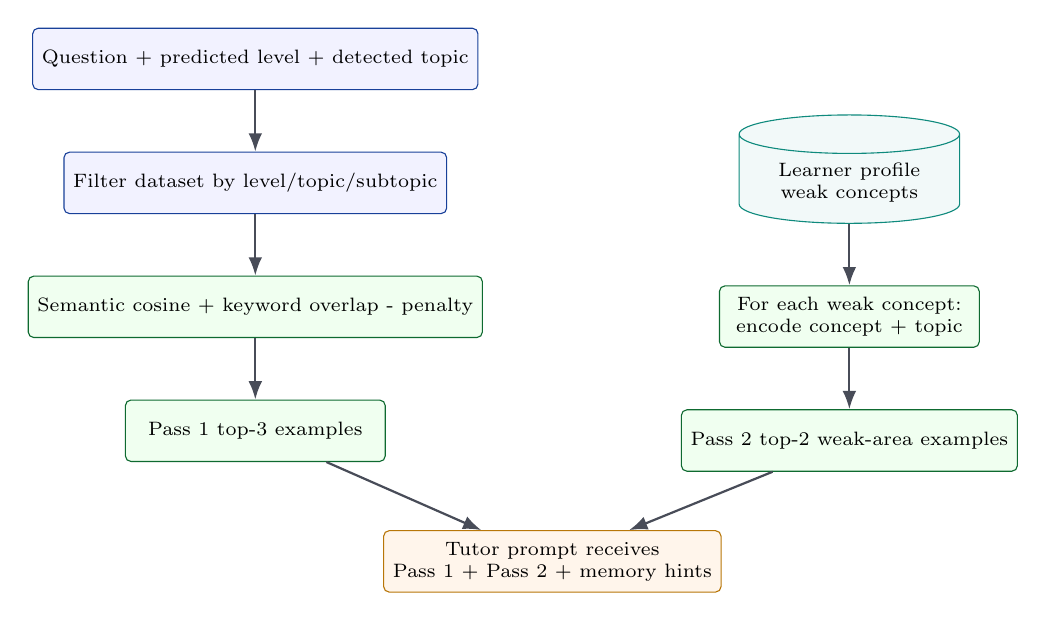
\begin{tikzpicture}[node distance=0.78cm]
\node[proc] (query) {Question + predicted level + detected topic};
\node[proc, below=of query] (filter) {Filter dataset by level/topic/subtopic};
\node[data, below=of filter] (score) {Semantic cosine + keyword overlap - penalty};
\node[data, below=of score] (pass1) {Pass 1 top-3 examples};
\node[store, right=3.7cm of filter] (profile) {Learner profile\\weak concepts};
\node[data, below=of profile] (weakquery) {For each weak concept:\\encode concept + topic};
\node[data, below=of weakquery] (pass2) {Pass 2 top-2 weak-area examples};
\node[agent, below=1.2cm of $(pass1)!0.5!(pass2)$] (tutor) {Tutor prompt receives\\Pass 1 + Pass 2 + memory hints};
\draw[arrow] (query) -- (filter);
\draw[arrow] (filter) -- (score);
\draw[arrow] (score) -- (pass1);
\draw[arrow] (profile) -- (weakquery);
\draw[arrow] (weakquery) -- (pass2);
\draw[arrow] (pass1) -- (tutor);
\draw[arrow] (pass2) -- (tutor);
\end{tikzpicture}}
\caption{Two-pass RAG: query relevance plus personalized weak-area retrieval.}
\end{figure}

\subsection{RAG Evaluation Results}

The current repository stores a reproducible 18-question RAG evaluation checkpoint. The saved report states \texttt{RAG\_TOP\_N=3}. The main results are:

\begin{table}[H]
\centering
\begin{tabular}{lrl}
\toprule
\textbf{Layer} & \textbf{Metric} & \textbf{Saved checkpoint} \\
\midrule
Retrieval & Hit Rate@3 & 83.3\% \\
Retrieval & MRR & 0.8333 \\
Retrieval & Topic Precision & 83.3\% \\
Retrieval & Level Precision & 100.0\% \\
Retrieval & Average Semantic Similarity & 0.7153 \\
Retrieval & Level Detection Accuracy in RAG sample & 77.8\% \\
Generation & Faithfulness & 5.00 / 5 \\
Generation & Answer Relevancy & 5.00 / 5 \\
Generation & Context Utilization & 4.44 / 5 \\
Generation & Level Fit & 4.94 / 5 \\
\bottomrule
\end{tabular}
\caption{Saved RAG evaluation checkpoint.}
\label{tab:rag-current}
\end{table}


\begin{cautionbox}
A later summarized evaluation run reports a stronger retrieval scorecard (Hit Rate@3 = 88.9\%, MRR = 0.8889, Topic Precision = 88.9\%, Level Precision = 100\%, and Average Semantic Similarity = 0.7172). The conservative values in Table~\ref{tab:rag-current} are retained as the primary checkpoint because they are tied to the saved per-question evaluation artifacts.
\end{cautionbox}

\subsection{Weak-Area Retrieval Results}

The repository also stores \texttt{eval/pass2\_eval\_results.json}. It evaluates five simulated learner weakness profiles across backpropagation, RNNs, overfitting, attention, and CNNs. Results:

\begin{table}[H]
\centering
\footnotesize
\begin{tabularx}{\textwidth}{>{\raggedright\arraybackslash}p{0.31\textwidth}p{0.13\textwidth}Y}
\toprule
\textbf{Metric} & \textbf{Value} & \textbf{Interpretation} \\
\midrule
Profiles evaluated & 5 & Five different topic/weak-concept configurations. \\
Retrieved examples per profile & 2 & Exactly two examples returned per case. \\
Keyword relevance & 100\% & Retrieved examples contained weak-area concepts. \\
Average semantic similarity & 0.4931 & Moderate similarity is expected because weak concepts are short queries. \\
\bottomrule
\end{tabularx}
\caption{Pass-2 personalized weak-area retrieval evaluation.}
\end{table}

Examples include retrieving chain-rule and gradient-flow backpropagation examples, pooling and feature-map CNN examples, and attention-score/QKV examples for advanced attention weaknesses.

% =========================================================
\section{Tutor Agent and Prompting Strategy}

\subsection{Tutor Prompt Assembly}

The Tutor Agent uses the classifier level, detected topic, retrieved examples, weak-area examples, memory hint, evaluation strategy hint, and teaching mode. The updated code explicitly separates a system instruction from the user prompt.

\subsubsection{Tutor System Message}

\begin{lstlisting}
You are EduAgent, an adaptive AI tutor specializing in {topic}.
You MUST stay focused on {topic} throughout your answer.
Do not drift into unrelated ML concepts unless {topic} itself explicitly requires them.
Pitch your explanation at {level} level.
\end{lstlisting}

\subsubsection{Tutor User Prompt Template}

\begin{lstlisting}
QUESTION: {user_question}
TOPIC: {topic}{memory_section}{eval_section}

RETRIEVED KNOWLEDGE BASE EXAMPLES - these are your PRIMARY source:
{examples_text}{weak_rag_section}

GROUNDING RULES (follow strictly):
1. Build your answer directly upon the facts, concepts, and explanations in the retrieved examples above.
2. Every key claim in your answer should trace back to the retrieved examples.
3. You may expand or re-explain retrieved content - but do NOT ignore it.
4. Do NOT copy retrieved text verbatim - synthesize and adapt in your own words.
5. Do NOT introduce facts or concepts that contradict the retrieved examples.
6. Do NOT include citation markers or bracketed source references such as [1], [2], or [3].

LEVEL GUIDE:
- beginner: simple words, analogies, no jargon
- intermediate: moderate detail, 1-2 key terms explained
- advanced: technical depth, assume background knowledge

ANSWER FORMAT:
- Use short bullet points.
- Start with the direct answer in the first bullet.
- Use 3 to 5 bullets total.
- Keep each bullet to 1 or 2 short sentences.
- Add a final "Next step:" bullet only when a useful follow-up topic naturally fits.
- Do not use numbered citations, footnotes, or source brackets.

{mode_instruction}
Answer clearly and concisely in the bullet format above.
\end{lstlisting}

\subsection{Adaptive Teaching Modes}

\subsubsection{Mode Selection Logic}

Mode selection prioritizes the latest same-topic evaluation hint. If no same-topic hint exists, it falls back to profile mastery, weak areas, and topic counts.

\begin{figure}[H]
\centering
\resizebox{0.92\textwidth}{!}{%
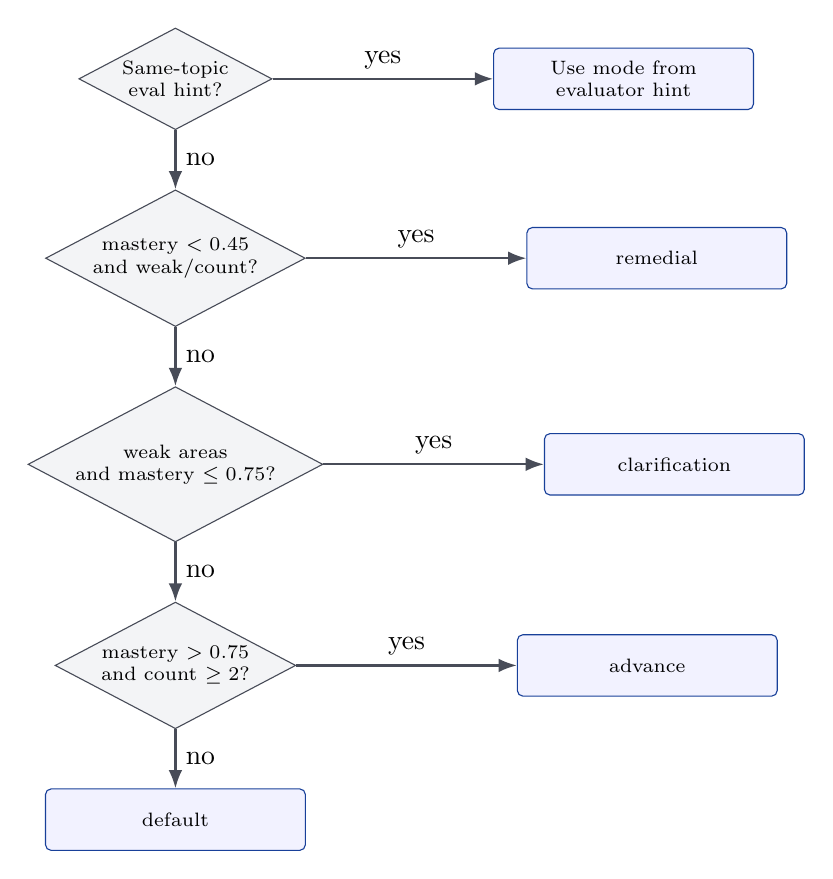
\begin{tikzpicture}[node distance=0.75cm]
\node[decision] (eval) {Same-topic\\eval hint?};
\node[proc, right=2.8cm of eval] (evalmode) {Use mode from\\evaluator hint};
\node[decision, below=of eval] (rem) {mastery $<0.45$\\and weak/count?};
\node[proc, right=2.8cm of rem] (remedial) {remedial};
\node[decision, below=of rem] (clar) {weak areas\\and mastery $\le0.75$?};
\node[proc, right=2.8cm of clar] (clarification) {clarification};
\node[decision, below=of clar] (adv) {mastery $>0.75$\\and count $\ge2$?};
\node[proc, right=2.8cm of adv] (advance) {advance};
\node[proc, below=of adv] (default) {default};
\draw[arrow] (eval) -- node[above]{yes} (evalmode);
\draw[arrow] (eval) -- node[right]{no} (rem);
\draw[arrow] (rem) -- node[above]{yes} (remedial);
\draw[arrow] (rem) -- node[right]{no} (clar);
\draw[arrow] (clar) -- node[above]{yes} (clarification);
\draw[arrow] (clar) -- node[right]{no} (adv);
\draw[arrow] (adv) -- node[above]{yes} (advance);
\draw[arrow] (adv) -- node[right]{no} (default);
\end{tikzpicture}}
\caption{Teaching-mode inference in the updated Tutor Agent.}
\end{figure}

\subsubsection{Mode-Specific Instruction Blocks}

\paragraph{Remedial mode.}
\begin{lstlisting}
Mode-specific instructions:
- Re-teach from scratch.
- Use very simple wording.
- Use one small concrete example.
- Explain in 4 to 6 short sentences.
- Focus on one main idea first before adding detail.
- Avoid abstract definitions unless absolutely necessary.
- Avoid repeating the same explanation style or analogy used earlier for this topic.
- Start with: "Let's simplify it completely."
\end{lstlisting}

\paragraph{Clarification mode.}
\begin{lstlisting}
Mode-specific instructions:
- Briefly restate the main idea in one or two simple sentences.
- Then focus on the weak or confusing concept.
- Use one clear example.
- Do not repeat the whole long explanation.
- Keep the answer focused and moderately short.
\end{lstlisting}

\paragraph{Advance mode.}
\begin{lstlisting}
Mode-specific instructions:
- Assume the learner understood the basics.
- Avoid repeating the full beginner introduction.
- Give a slightly deeper explanation.
- Connect the concept to a related next-step idea.
- Keep the answer clear but more intellectually rich.
\end{lstlisting}

\paragraph{Default mode.}
\begin{lstlisting}
Mode-specific instructions:
- Give a normal level-appropriate explanation.
\end{lstlisting}

\subsection{LLM Backend and Fallback}

The updated repository uses Gemini through \texttt{google.generativeai}. \texttt{agents/llm\_client.py} accepts OpenAI-style message dictionaries, maps them into Gemini roles, passes system text as \texttt{system\_instruction}, and retries with exponential backoff. Rate-limit/quota errors are detected, and after repeated failures the session marks quota exhausted so later calls return fallback content immediately. Tutor fallback answers are generated from retrieved examples only; the code avoids injecting unrelated canned explanations.

% =========================================================
\section{Evaluator Agent}

\subsection{Follow-Up Question Prompt}

The Evaluator Agent asks a short conceptual follow-up question after each tutor answer.

\begin{lstlisting}
You are an evaluator for an adaptive AI tutor.

Topic: {topic}
Learner level: {level}

Original learner question:
{user_question}

Tutor's answer:
{tutor_answer}

Generate ONE short follow-up question to test whether the learner understood the main idea.

Rules:
- Match the learner's level.
- Focus on conceptual understanding, not memorization.
- Keep it short and clear.
- Return only the question.
\end{lstlisting}

If the tutor answer is a local fallback, the evaluator uses a safe hardcoded fallback: \textit{In your own words, what is the main idea from the explanation?}

\subsection{Reply Evaluation Prompt}

\begin{lstlisting}
You are an evaluator for an adaptive AI tutor.

Topic: {topic}
Learner level: {level}

Follow-up question:
{followup_question}

Learner reply:
{learner_reply}

Evaluate the learner's reply.

Return valid JSON only with exactly these keys:
- understanding_level: one of ["good", "partial", "poor"]
- weak_concepts: list of short concept names
- feedback: short educational feedback
- recommended_action: one of ["advance", "re-explain", "give easier example", "give more practice"]

Rules:
- Be fair and educational.
- If the learner is partly correct, mark as "partial".
- Keep weak_concepts short and specific.
- Do not include markdown.
- Return valid JSON only.
\end{lstlisting}

The output is validated with a Pydantic \texttt{EvaluationResult} schema before it can update the profile. If parsing fails, the system returns a safe \texttt{partial} result rather than incorrectly pushing the learner into remedial mode.

% =========================================================
\section{Memory Agent and Personalization}

\subsection{Profile Schema}

The Memory Agent normalizes every profile to contain:

\begin{lstlisting}
sessions, questions_asked, last_level, level_history,
topics_seen, topic_counts, weak_areas, mastery,
used_explanations, recommended_next_topics, last_evaluation
\end{lstlisting}

It also includes backward-compatibility logic for older profile shapes, such as converting an old list of weak areas into a topic-to-concept dictionary.

\subsection{Mastery Update Model}

The updated Memory Agent uses a named heuristic mastery model with initial score $m_0=0.5$:

\begin{align}
\text{good:}\quad & m \leftarrow \min(1.0,\; m + 0.20(1-m)) \\
\text{partial:}\quad & m \leftarrow \max(0.0,\; m - 0.06) \\
\text{poor:}\quad & m \leftarrow \max(0.0,\; m - 0.18)
\end{align}

The good-update rule has diminishing returns: a learner at 0.50 gains 0.10, while a learner at 0.90 gains only 0.02.

\subsection{Weak-Area Logic}

\begin{itemize}
    \item \textbf{Good evaluation:} clears all weak areas for the topic if no specific concepts are flagged, or removes only the resolved concepts if the evaluator names them.
    \item \textbf{Partial/poor evaluation:} accumulates evaluator-provided weak concepts.
    \item \textbf{Repeated revisits:} if a topic is visited at least three times with no weak concept identified, the system adds \texttt{core understanding} as a weak signal.
\end{itemize}

\subsection{Memory Hint Strings}

The memory hint is purely deterministic profile logic, not an LLM call. It can include these lines depending on the profile:

\begin{lstlisting}
The learner has seen this topic before. Do not restart with the exact same beginner introduction.
The learner has previously struggled with: {concepts}. Address these concepts carefully.
The learner appears weak in this topic. Use simpler wording, intuition, and one concrete example.
The learner appears comfortable with this topic. You may go slightly deeper than before.
Avoid repeating the exact same prior explanation style if possible. Previously used: {tags}.
No strong prior history for this topic. Start with a clear explanation.
\end{lstlisting}

\subsection{Evaluation Strategy Hint Strings}

Strategy hints fire only when \texttt{last\_evaluation["topic"]} matches the current topic. This prevents old feedback from unrelated topics from contaminating new explanations.

\begin{lstlisting}
Teaching mode: remedial. The learner did not understand the previous explanation. Do NOT repeat the same analogy-driven explanation. Re-teach from scratch using very simple wording, one tiny concrete example, and a short step-by-step explanation.

Teaching mode: clarification. The learner understood partially. Do not repeat the whole answer. Briefly restate the core idea, then focus on the confusing part with one clear example.

Teaching mode: advance. The learner understood the previous explanation well. Do not repeat the full beginner introduction. Give a slightly deeper explanation and connect it to the next related concept.
\end{lstlisting}

Recommended-action addenda can then request an easier example, re-explanation, more practice, or advancement to the next topic.

% =========================================================
\section{Application Layer, Security, and Voice}

\subsection{Gradio Application}

The UI uses Gradio with a polished dark theme, authenticated workspace, chat panel, follow-up panel, retrieved-example display, pipeline insights, profile cards, and charts. The charts visualize mastery by topic, topic revisit count, and weak concept count by topic. The \texttt{app/main.py} callbacks orchestrate asking a question, updating the profile, generating a follow-up, evaluating the reply, and refreshing UI state.

\subsection{Authentication and Storage}

Passwords are not stored directly. \texttt{auth/password\_utils.py} uses:

\begin{itemize}
    \item \texttt{os.urandom(16)} for salt generation,
    \item PBKDF2-HMAC-SHA256 with 200,000 iterations,
    \item base64 encoding of \texttt{salt || hash},
    \item \texttt{hmac.compare\_digest} for timing-safe verification.
\end{itemize}

SQLite uses WAL mode and \texttt{synchronous=NORMAL}. Profile fields such as weak areas, mastery, topics seen, and recommendations are stored as JSON strings and loaded with safe defaults if corrupted or missing.

\subsection{Voice Interaction}

The updated repository includes a \texttt{voice/} module:

\begin{itemize}
    \item \texttt{speech\_to\_text.py}: Whisper-based transcription wrapper using \texttt{openai-whisper}, \texttt{librosa}, and confidence derived from segment log-probabilities.
    \item \texttt{text\_to\_speech.py}: TTS wrapper that tries Piper if installed and falls back to local \texttt{pyttsx3} synthesis.
    \item \texttt{utils.py}: Gradio-facing glue functions for transcription and synthesis.
\end{itemize}

Voice features improve accessibility and demonstration value but are not required for the core tutoring loop.

% =========================================================
\section{Evaluation Evidence}

\subsection{Classifier Evaluation}

The strongest quantitative result is the DistilBERT classifier: 97.92\% accuracy and 97.91\% macro-F1 on the balanced 240-row test split. This justifies replacing the earlier heuristic-only difficulty detection with a fine-tuned classifier plus lightweight calibration.

\subsection{Dataset Evaluation}

Dataset analysis shows that \texttt{eduagent\_dataset\_easy\_v2.csv} is stronger for educational tutoring because it has 2,400 rows, 19 columns, richer metadata, more answer vocabulary, reasoning expectations, learner-confusion annotations, and no duplicate questions or answers. The 900-row baseline dataset remains useful for lightweight baseline experimentation.

\subsection{RAG Evaluation}

The saved evaluation checkpoint reports strong generation quality even though retrieval still has room for improvement. It shows perfect level precision in retrieved examples but topic retrieval misses in a few cases, especially where semantically adjacent topics overlap. This is an important finding: generation can be highly faithful to the provided context while topic detection/retrieval still requires refinement.

\subsection{Personalization Evaluation}

The saved personalization evaluation compares a clean baseline profile against a simulated experienced learner profile. It evaluates 10 questions and reports that teaching mode changed in 3/10 cases, while level detection did not change. This means personalization affects the teaching strategy rather than artificially changing the learner's predicted level. Examples include baseline \texttt{default} mode changing to \texttt{clarification} for gradient descent, vanishing gradient, and backpropagation questions based on learner memory.

\subsection{Unit Tests}

The submitted repository unit-test suite reports:

\begin{lstlisting}
51 passed in 1.85s
\end{lstlisting}

The tests cover authentication behavior, password hashing/verification, email validation, registration edge cases, profile normalization, backward compatibility, mastery clamping, diminishing returns, weak-area update behavior, and used-explanation deduplication.


\begin{table}[H]
\centering
\footnotesize
\begin{tabularx}{\textwidth}{>{\ttfamily\raggedright\arraybackslash\footnotesize}p{0.25\textwidth}Y Y}
\toprule
\textbf{Test file} & \textbf{Observed scope} & \textbf{Main behavior covered} \\
\midrule
\texttt{tests/test\_auth.py} & Auth/security & Password verification, hash uniqueness, invalid email handling, duplicate-user path, and registration/login edge cases. \\
\texttt{tests/test\_memory.py} & Personalization & Topic counts, mastery deltas, weak-area updates, used-explanation tags, hint generation, clamping, and diminishing-returns behavior. \\
\texttt{tests/test\_profile.py} & Profile schema & Default keys, type repair, legacy weak-area conversion, profile idempotency, and JSON round-trip behavior. \\
\bottomrule
\end{tabularx}
\caption{Unit-test coverage areas.}
\label{tab:unit-tests}
\end{table}

% =========================================================
\section{Comparison Against Baselines}

\subsection{Dataset Baseline}

\begin{table}[H]
\centering
\begin{tabular}{lcc}
\toprule
\textbf{Criterion} & \textbf{Baseline dataset} & \textbf{Updated dataset} \\
\midrule
Rows & 900 & 2,400 \\
Columns & 5 & 19 \\
Subtopics & absent/limited & explicit \\
Pedagogical annotations & low & high \\
RAG readiness & moderate & high \\
Instruction tuning usefulness & moderate & stronger \\
\bottomrule
\end{tabular}
\caption{Qualitative comparison of the baseline and updated datasets.}
\end{table}

\subsection{Classifier Baseline}

The classifier is compared against simple non-neural baselines: a majority-class predictor and a keyword-heuristic predictor. The fine-tuned DistilBERT model is the deployed classifier in the updated application.

\begin{table}[H]
\centering
\begin{tabular}{lcc}
\toprule
\textbf{Method} & \textbf{Accuracy} & \textbf{Macro-F1} \\
\midrule
Majority class baseline & 33.3\% & 16.7\% \\
Keyword heuristic baseline & 62.1\% & 60.4\% \\
Fine-tuned DistilBERT & 97.92\% & 97.91\% \\
\bottomrule
\end{tabular}
\caption{Classifier comparison against simple non-neural baselines.}
\end{table}


\subsection{Personalization Baseline}

The personalization baseline evaluates whether stored learner history changes tutoring strategy without changing classifier output. The clean profile acts as the baseline; the personalized profile simulates an eight-session learner history with stored weak areas and topic counts. In the saved evaluation, 3 out of 10 teaching-mode decisions changed, while difficulty-level detection remained stable in all 10 cases.

\begin{table}[H]
\centering
\scriptsize
\begin{tabularx}{\textwidth}{>{\raggedright\arraybackslash}p{0.29\textwidth}p{0.13\textwidth}p{0.15\textwidth}p{0.10\textwidth}Y}
\toprule
\textbf{Question} & \textbf{Baseline mode} & \textbf{Personalized mode} & \textbf{Level changed?} & \textbf{Observed personalization signal} \\
\midrule
What is gradient descent? & default & clarification & No & Prior gradient-descent history triggers focused clarification instead of a fresh default explanation. \\
How does a neural network learn? & default & default & No & No mode change; the memory state did not indicate a targeted weakness for this prompt. \\
What is the vanishing gradient problem? & default & clarification & No & Prior gradient-related weakness shifts the answer toward clarifying gradient-flow failure. \\
Explain the attention mechanism in transformers. & default & default & No & No mode change; topic memory did not require remediation. \\
What is overfitting and how do you fix it? & default & default & No & Default mode retained because profile state did not demand weak-area remediation. \\
How does backpropagation work? & default & clarification & No & Stored weak concepts such as chain rule and gradient flow trigger clarification mode. \\
What is the difference between supervised and unsupervised learning? & default & default & No & Classifier and mode remain stable for a general ML comparison. \\
What is a convolutional neural network used for? & default & default & No & No personalization shift was needed for this first-level CNN question. \\
How does the Adam optimizer improve on SGD? & default & default & No & No teaching-mode change; topic detection requires future refinement for this case. \\
What is transfer learning and when should you use it? & default & default & No & Default mode retained; no stored transfer-learning weakness was activated. \\
\midrule
\textbf{Summary} & \textbf{default-only baseline} & \textbf{3/10 changed} & \textbf{0/10} & Memory changes teaching strategy in targeted cases while preserving classifier stability. \\
\bottomrule
\end{tabularx}
\caption{Personalized profile vs. clean-profile baseline evaluation.}
\label{tab:personalization-baseline}
\end{table}

\subsection{Plain LLM Tutor vs EduAgent}


\begin{table}[H]
\centering
\scriptsize
\begin{tabularx}{\textwidth}{>{\raggedright\arraybackslash}p{0.34\textwidth}Y Y}
\toprule
\textbf{Capability} & \textbf{Plain LLM tutor} & \textbf{EduAgent} \\
\midrule
Difficulty classification & No explicit trained classifier & DistilBERT + calibration \\
Topic detection & implicit & alias + semantic cosine + fallback \\
Retrieval grounding & optional/manual & two-pass RAG over dataset \\
Learner memory & usually stateless & SQLite profile with mastery and weak areas \\
Follow-up evaluation & not automatic & Evaluator Agent + Pydantic validation \\
Adaptive mode selection & not explicit & default/remedial/clarification/advance \\
Progress dashboard & absent & Gradio profile + charts \\
Voice input/output & absent unless separately built & Whisper + TTS wrappers \\
\bottomrule
\end{tabularx}
\caption{System comparison against a plain LLM question-answering tutor.}
\end{table}

% =========================================================
\section{Deployment Considerations}

For a deployed product, ordinary learners should not need to provide Gemini, Groq, OpenAI, or Ollama credentials. In the updated repository, API access is configured on the backend through environment variables such as \texttt{GEMINI\_API\_KEY}. Users interact only with the web UI. Ollama or local model options are best treated as developer/institutional fallback paths, not as end-user requirements.

\begin{cautionbox}
\textbf{Production note.} API keys must never be hardcoded or committed. They should live in \texttt{.env} for local development and in managed secrets/environment variables for deployment. The repository already contains \texttt{.env.example} and uses \texttt{python-dotenv}/environment variables.
\end{cautionbox}

A production-grade version would require rate limiting, usage monitoring, admin controls, cost limits, data privacy policy, and stronger evaluation on real learner data.

% =========================================================
\section{Limitations and Threats to Validity}

\begin{enumerate}
    \item \textbf{Synthetic dataset:} The 2,400-row dataset is generated with Gemini and deterministic filters. It is structured and useful, but it is still synthetic rather than collected from real learners.
    \item \textbf{Classifier generalization:} The 97.92\% test accuracy is on an in-distribution split of the same generated dataset. Real student wording, spelling errors, and incomplete questions may reduce performance.
    \item \textbf{RAG sample size:} The current repository RAG checkpoint has 18 questions. This is useful for project evidence but not enough for publication-level statistical confidence.
    \item \textbf{LLM-as-judge bias:} Generation scores use an LLM judge. This is practical for tutoring quality but should be supplemented with human evaluation.
    \item \textbf{Mastery heuristic:} Mastery updates are interpretable but not yet calibrated against real learning gains or Bayesian Knowledge Tracing.
    \item \textbf{Weak-area persistence:} Weak concepts accumulate unless resolved; future versions should add decay or recency weighting.
    \item \textbf{API dependency:} Tutor/evaluator quality depends on the configured LLM backend and quota availability.
\end{enumerate}

% =========================================================
\section{Future Work}

\begin{itemize}
    \item Add a larger human-evaluated test set of real learner questions.
    \item Calibrate mastery updates with Bayesian Knowledge Tracing or Item Response Theory.
    \item Add weak-concept decay and time-aware learning history.
    \item Extend RAG evaluation from 18 examples to a 100+ question benchmark across all 25 topics.
    \item Add teacher/admin dashboard for classroom-level analytics.
    \item Support document/PDF upload as a separate RAG corpus while keeping the dataset-based RAG as the stable baseline.
    \item Add multimodal diagram-question input using a vision-capable model.
    \item Package backend API keys as deployment-side secrets so students never need to configure model providers.
\end{itemize}

% =========================================================
\section{Conclusion}

EduAgent is an impressive academic prototype because it integrates several components that are often presented separately: dataset construction, fine-tuned NLP classification, semantic retrieval, adaptive prompting, learner memory, evaluation, authentication, dashboarding, and voice interaction. The updated repository's strongest quantitative evidence is the fine-tuned DistilBERT classifier with 97.92\% accuracy and 97.91\% macro-F1 on a balanced 240-row test set. The two-pass RAG evaluation shows strong grounding and level fit, while revealing remaining topic-detection/retrieval issues that are appropriate future-work targets. The Memory Agent closes the loop by converting evaluator output into mastery updates, weak-area tracking, teaching modes, and future prompt hints. Overall, EduAgent is best described as a personalized, agentic, retrieval-augmented AI tutoring system for AI/ML education, suitable as a strong B.Tech GenAI project and a foundation for further educational AI research.

\newpage
\appendix

% =========================================================
\section{Appendix A: RAG Judge Prompt}

The RAG evaluation script uses a combined LLM-as-judge prompt:

\begin{lstlisting}
Rate this AI tutor response on 4 dimensions (1=worst, 5=best).

QUESTION: {question}
STUDENT LEVEL: {level}
RETRIEVED CONTEXT (what the tutor was given):
{ctx}
TUTOR ANSWER: {answer}

Scoring criteria:
- faithfulness: answer only states things supported by the context (not hallucinated)
- relevancy: answer directly and fully addresses the question
- context_use: tutor explicitly built upon or referenced the retrieved examples
- level_fit: language and depth suit a {level} student

Reply ONLY with this JSON (integers 1-5, no other text):
{"faithfulness": <1-5>, "relevancy": <1-5>, "context_use": <1-5>, "level_fit": <1-5>, "reason": "<one sentence>"}
\end{lstlisting}

% =========================================================
\section{Appendix B: Core Equations}

\subsection{Retrieval Ranking}
\[
\text{final\_score} = 0.75 \cdot \cos(q, d_i) + 0.25 \cdot \text{Jaccard}_{1,2}(q,d_i) - \text{penalty}(d_i)
\]

\subsection{Mastery Update}
\[
\begin{array}{ll}
\text{good:} & m \leftarrow \min(1.0, m + 0.20(1-m)) \\
\text{partial:} & m \leftarrow \max(0.0, m - 0.06) \\
\text{poor:} & m \leftarrow \max(0.0, m - 0.18)
\end{array}
\]

% =========================================================
\section{Appendix C: Selected Reproducibility Commands}

\begin{lstlisting}[language=bash]
# Run unit tests
python -m pytest -q tests

# Train the difficulty classifier
python train_distilbert_difficulty.py \
  --data_path datasets/data_easy/eduagent_dataset_easy_v2.csv \
  --output_dir models/distilbert_eduagent_v2 \
  --epochs 3 \
  --batch_size 8

# Run RAG evaluation
python rag_evaluation.py --n 18

# Run the application
python gradio_app.py
\end{lstlisting}

% =========================================================
\section*{References}
\begin{enumerate}
    \item S. Yao et al. \textit{ReAct: Synergizing Reasoning and Acting in Language Models}. ICLR, 2023.
    \item V. Sanh et al. \textit{DistilBERT, a distilled version of BERT: smaller, faster, cheaper and lighter}. NeurIPS EMC2 Workshop, 2019.
    \item N. Reimers and I. Gurevych. \textit{Sentence-BERT: Sentence Embeddings using Siamese BERT-Networks}. EMNLP, 2019.
    \item P. Lewis et al. \textit{Retrieval-Augmented Generation for Knowledge-Intensive NLP Tasks}. NeurIPS, 2020.
    \item A. Corbett and J. Anderson. \textit{Knowledge Tracing: Modeling the Acquisition of Procedural Knowledge}. User Modeling and User-Adapted Interaction, 1994.
    \item J. Devlin et al. \textit{BERT: Pre-training of Deep Bidirectional Transformers for Language Understanding}. NAACL, 2019.
\end{enumerate}

\end{document}
